\documentclass{anstrans}
%%%%%%%%%%%%%%%%%%%%%%%%%%%%%%%%%%%
\title{Residual Monte Carlo Transport in Time with Consistent Low-Order Acceleration for
    1D Thermal Radiative Transfer}
\author{Simon R.~Bolding and Jim E.~Morel}

\institute{Texas A\&M University Nuclear Engineering Department, 
}

\email{sbolding@tamu.edu \and morel@tamu.edu}

% Optional disclaimer: remove this command to hide
%\disclaimer{Notice: this manuscript is a work of fiction. Any resemblance to
%actual articles, living or dead, is purely coincidental.}

%%%% packages and definitions (optional)
\usepackage{graphicx} % allows inclusion of graphics
\usepackage{booktabs} % nice rules (thick lines) for tables
\usepackage{microtype} % improves typography for PDF
\usepackage{comment}
\usepackage{float}

\newcommand{\SN}{S$_N$}
\renewcommand{\vec}[1]{\bm{#1}} %vector is bold italic
\newcommand{\vd}{\bm{\cdot}} % slightly bold vector dot
\newcommand{\grad}{\vec{\nabla}} % gradient
\newcommand{\ud}{\mathop{}\!\mathrm{d}} % upright derivative symbol
\renewcommand{\eqref}[1]{(\ref{#1})}
\renewcommand*\thetable{\Roman{table}}
\usepackage{caption}

\captionsetup[table]{labelsep=period}
\captionsetup[figure]{labelsep=period}
\newcommand{\N}{\mathbb{N}}
\newcommand{\Z}{\mathbb{Z}}
\newcommand{\deriv}[2]{\frac{\mathrm{d} #1}{\mathrm{d} #2}}
\newcommand{\pderiv}[2]{\frac{\partial #1}{\partial #2}}
\newcommand{\bx}{\mathbf{X}}
\newcommand{\ba}{\mathbf{A}}
\newcommand{\by}{\mathbf{Y}}
\newcommand{\bj}{\mathbf{J}}
\newcommand{\bs}{\mathbf{s}}
\newcommand{\B}[1]{\ensuremath{\mathbf{#1}}}
\newcommand{\Dt}{\Delta t}
\renewcommand{\d}{\mathrm{d}}
\newcommand{\mom}[1]{\langle #1 \rangle}
\newcommand{\xl}{{x_{i-1/2}}}
\newcommand{\xr}{{x_{i+1/2}}}
\newcommand{\il}{{i-1/2}}
\newcommand{\ir}{{i+1/2}}
\newcommand{\keff}{\ensuremath{k_{\text{eff}}}}
\newcommand{\sig}[1]{\ensuremath{\Sigma_{#1}}}
\newcommand{\ra}{\ensuremath{\rightarrow}}
\newcommand{\dd}{\ensuremath{\mathrm{d}}}
\renewcommand{\O}{\ensuremath{\mathbf{\Omega}}}
\newcommand{\adj}{\ensuremath{{}^{\dagger}}}
\newcommand{\x}{\ensuremath{\mathbf{x}}}
\newcommand{\T}{\ensuremath{\text{T}}}
\newcommand{\iso}[2]{$^{#2}$#1}
\newcommand{\phibar}{\ensuremath{\overline{\phi}}}
\newcommand{\cur}[1]{\left\{ #1 \right\}}
\newcommand{\jl}{{j-1/2}}
\newcommand{\jr}{{j+1/2}}
\newcommand{\E}[1]{\ensuremath{\operatorname{E}_{#1}}}
\newcommand{\rface}{\ensuremath{r_{\text{face}}}}
\newcommand{\FOM}{\ensuremath{\text{FOM}}}
\newcommand{\ds}[0]{\displaystyle}
\newcommand{\invcm}[0]{cm$^{-1}$}
\renewcommand{\u}[1]{\ensuremath{\underline{#1}}}
\newcommand{\dep}{\ensuremath{\delta\epsilon^{(m)}}}
\renewcommand{\ss}{\ensuremath{\|s\|}}
\newcommand{\pos}{{\text{pos}}}
\newcommand{\phsp}{\ensuremath{\left(\mathbf{r},\mathbf{\Omega},\nu,t\right)}}
\newcommand{\Del}{\ensuremath{\nabla}}


\begin{document}
%%%%%%%%%%%%%%%%%%%%%%%%%%%%%%%%%%%%%%%%%%%%%%%%%%%%%%%%%%%%%%%%%%%%%%%%%%%%%%%%
\section{Introduction}

Accurate solutions to the thermal radiative transfer (TRT) equations are important in the
high-energy, high-density physics regime, e.g., for inertial
confinement fusion and astrophysics simulations.  Moment-based hybrid Monte Carlo (MC)
methods have demonstrated great potential for accelerated
solutions to TRT problems~\cite{rmc,bolding_nse,holo_rh}.   These nonlinear acceleration methods iterate between a
high-order (HO) transport equation and a low-order (LO) system formulated with angular moments
and a fixed spatial mesh.  Physics operators that
are too expensive for the HO solver to resolve directly, e.g., photon absorption and emission,
are moved to the LO system. The lower-rank LO equations can be solved with Newton
methods to allow for non-linearities in the LO equations to be efficiently
resolved.  The high-order (HO) problem is defined by the radiation transport equation with
sources computed with the previous LO solution. A MC transport solution to the HO
problem is used to construct consistency terms that appear in the LO equations. These consistency terms preserve the accuracy of the HO
solution in the next LO solve.

Previously, residual Monte Carlo (RMC) methods have been used to provide efficient
solution to the HO transport problem~\cite{rmc,bolding_nse}; high-fidelity solutions,
with minimal statistical noise, have been achieved for problems with optically-thick, diffusive
regions that lead to slowly varying
solutions.  However, the results in these works used a backward
Euler (BE) discretization for the time variable, which can inaccurately disperse radiation
wavefronts in optically thin problems. We have extended the work
in~\cite{bolding_nse} to include higher-accuracy MC treatment of the time variable for the
radiation unknowns. The exponentially-convergent Monte Carlo (ECMC)
algorithm was modified to include integration of the time variable;
this includes the introduction of a step, doubly-discontinuous (SDD) trial space representation
in time.  A new
parametric closure of the LO equations, introducing additional time-closure consistency
terms, was derived to capture the time accuracy of the HO
ECMC simulations.  The LO equations can preserve the accuracy of MC radiation transport treatment in
time, with the same numerical expense as Backward Euler (BE) time-discretized S$_2$
equations. 
%We have derived the LO equations directly from the transport equation,
%such that, neglecting spatial discretization differences,
%the HO and LO solutions are consistent upon convergence.
Herein we briefly describe the algorithm, and we present results for
one-dimensional (1D), grey test problems.  We compare our method to the implicit MC
(IMC) method~\cite{fnc}, the standard MC solution
method for TRT problems.

%%%%%%%%%%%%%%%%%%%%%%%%%%%%%%%%%%%%%%%%%%%%%%%%%%%%%%%%%%%%%%%%%%%%%%%%%%%%%%%%
\section{Acknowledgments}

This research was supported with funding received from the DOE National
Nuclear Security Administration, under Award Number(s) DE-NA0002376. 

%%%%%%%%%%%%%%%%%%%%%%%%%%%%%%%%%%%%%%%%%%%%%%%%%%%%%%%%%%%%%%%%%%%%%%%%%%%%%%%%
\section{Methodology}
The 1D, grey TRT equations consist of the radiation and
material energy balance equations, i.e.,\vspace{-0.05in}
\begin{align}\label{ho_cont}
    \frac{1}{c}\pderiv{I(x,\mu,t)}{t} + \mu \pderiv{I(x,\mu,t)}{x} &+ \sigma_a
    I(x,\mu,t)
= \frac{1}{2} \sigma_a a c T^4(x,t)
    \\ \label{t_cont}
  \rho c_v \pderiv{T(x,t)}{t} &=  \sigma_a \phi(x,t) - \sigma_a a c T^4(x,t),
\end{align}
where physical scattering could optionally be included in Eq.~\eqref{ho_cont}, and
appropriate initial and boundary conditions are specified.
In the above equations $x$ is the position, $t$ is the time, $\mu$ is
the $x$-direction cosine of the angular intensity $I(x,\mu,t)$, $\sigma_a$ is the
macroscopic absorption cross section (cm$^{-1}$), and $a$, $c$, $\rho$,
and
$c_v$ are the radiation constant, speed of light, mass density, and specific heat,
respectively.  The desired transient unknowns are the material
temperature $T(x,t)$ and the mean radiation intensity $\phi(x,t)=\int_{-1}^1
I(x,\mu,t) \d \mu$.  The mean intensity is related to the radiation energy density
$E_r$ by the relation $E_r = \phi/c$.  The equations can be 
strongly coupled through the gray Planckian emission source $\sigma_a a c T^4$, which
is a nonlinear function of temperature, and the absorption
term $\sigma_a \phi$.  

In our HOLO algorithm, the LO solver models isotropic scattering and
resolves the material temperature spatial distribution $T(x)$ over each time step, whereas
the HO solver computes weighted angular and temporal averages of $I(x,\mu,t)$.  The
fully-discrete LO equations are based on space-time-angle moments of the TRT equations, formed over a spatial finite-element (FE)
mesh.   Angularly, the LO
radiation equations are similar to S$_2$ equations,  with element-averaged
consistency parameters that are weighted averages of $\mu$. The BE time discretization is applied to emission source throughout, but the radiation
variables are left in terms of time-averaged and end-of-time-step unknowns.  This is analagous to
the time integration in IMC~\cite{fnc}.   Additional
consistency parameters are introduced in parametric closures that eliminate the auxillary
time-unknowns from the LO radiation equations.
If the angular and time
consistency parameters were estimated exactly, then the LO equations would exactly preserve HO moments,
neglecting spatial discretization error.  The consistency parameters are lagged
in each LO solve, estimated from the previous HO solution for $I(x,\mu,t)$,
as explained below.    The LO equations always conserve energy,
independent of the accuracy of the consistency terms.

The solution to the LO system is used to construct a spatially linear-discontinuous (LD) FE representation of
the emission source on the right hand side of Eq.~\eqref{ho_cont}.  This defines a fixed-source, pure absorber
transport problem for the HO operator. This HO transport problem is solved with the ECMC algorithm.  The ECMC
algorithm is an iterative RMC method that uses
batches of MC histories to estimate the error in the current trial-space estimate of 
$I(x,\mu,t)$.  It is noted that because we are not using
mesh adaptation in this work, exponential convergence in iterations cannot be maintained,
but reduced variance from the RMC formulation can still be achieved.  The output from ECMC is a projection $\tilde I(x,\mu,t)$ of the intensity onto
the chosen trial space. Once computed, $\tilde{I}(x,\mu)$ is used to directly evaluate the
necessary LO angular and time-closure consistency parameters.   The HO solution is not used to directly estimate a new temperature at
the end of the time step, which eliminates the need to linearize the emission source for
stability.

Iterations between the HO and LO solves can increase accuracy in strongly nonlinear
problems. However, for the problems tested here, only a single HO solve is performed during each
time step.  Thus, the HOLO algorithm, for the $n$'th time step, is
\begin{enumerate}
    \item Perform a LO solve to produce an initial guess for $T_{LO}^{n+1}(x)$
        and $\phi_{LO}^{n+1}(x)$, based on consistency terms estimated with
        $\tilde{I}^{n}(x,\mu)$ and a BE time
    discretization.
\item Solve the HO system for $\tilde{I}_{HO}(x,\mu,t)$ using ECMC, based on the current
    LO estimate of the emission and scattering sources.%$\sigma_s(T^k)\phi^{k}$ and $B(T)^{k}$.
\item Compute LO angular and time-closure consistency parameters with
    $\tilde{I}_{HO}(x,\mu,t)$.  
\item Solve the LO system using HO consistency parameters to produce a new
    estimate of $\phi^{n+1}_{LO}$ and $T^{n+1}_{LO}$.
\item Store $\tilde{I}^{n}(x,\mu)\leftarrow\tilde{I}^{n+1}(x,\mu)$, and move to the next time step.
\end{enumerate}

\subsection*{The LO System}
\label{sec:lo}

To derive the LO equations, we reduce the dimensionality of Eq.~\eqref{ho_cont} and
Eq.~\eqref{t_cont} by taking spatial, angular, and
temporal integrals.  The spatial moments are taken over each spatial cell $i$:
$x\in[x_{i-1/2},x_{i+1/2}]$, weighted with the standard linear Lagrange interpolatory FE basis functions.  For example, the left moment operator is defined by
\begin{equation}\label{x_mom}
    \mom{\cdot}_{L,i} = \frac{2}{h_i} \int_{x_{i-1/2}}^{\xr} b_{L,i}(x) (\cdot) \d x,
\end{equation}
where $h_i=x_{i+1/2}-x_{i-1/2}$ is the width of the spatial element and
$b_{L,i}(x)=(x_{i+1/2}-x)/h_i$ is the basis function corresponding to position
$x_{i-1/2}$. Angularly, the equations are integrated over the positive and negative half
ranges.  The angular integrals of the intensity are defined as $\phi^\pm(x) = \pm2\pi
\int_0^{\pm 1} I(x,\mu) \d \mu$.  Finally, the equations are integrated over the $n$'th
time step for $t\in[t^n,t^{n+1}]$ with width $\Delta t = t^{n+1}-t^{n}$.  

The positive half-range integral, $\mom{\cdot}_{L,i}$ moment, and
integration over a time step of Eq.~\eqref{ho_cont} yields
\begin{multline}\label{eq:t_moml_ex}
    \frac{\mom{\phi}_{L,i}^{+,n+1} - \mom{\phi}_{L,i}^{+,n}}{c \Delta t}
    -2\overline {\mu}_{i-1/2}^{\,+} \overline \phi_{i-1/2}^{\,+} + {\cur {\overline\mu}}_{L,i}^{+}
  \mom{\phibar}_{L,i}^{+}
  +  \cur{\overline\mu}_{R,i}^{+}
  \mom{\phibar}_{R,i}^{+} \\ +  \sigma_{a,i}^{n+1} h_i 
  \mom{\overline\phi}_{L,i}^{n+1,+}   = \frac{h_i}{2} \mom{\sigma_a^{n+1} a c T^{n+1,4}}_{L,i},
\end{multline}
where overlined quantities denote time averaging.  The time-averaged angular consistency
terms are approximated with the previous HO solution, e.g.,
\begin{equation}\label{const}
    \overline{\cur{{\mu}}}_{L,i}^+ =  \frac{
        {\displaystyle \frac{2}{h_i}} \int\limits_0^1 \int\limits_\xl^\xr \mu \, b_{L,i}(x)
        \overline{I}_{HO}(x,\mu) \d x \d \mu } 
{{\displaystyle \frac{2}{h_i}} \int\limits_0^1 \int\limits_\xl^\xr \, b_{L,i}(x)
\overline{I}_{HO}(x,\mu) \d x \d \mu } .
\end{equation}
where $\overline{I}(x,\mu)$ is a time-averaged LDFE projection in $x$ and $\mu$, as
explained in the next section.  For simplicity, the face terms are eliminated from the system using a LDFE
spatial approximation, with upwinding.  There is some inconsistency introduced in this approximation, but
it has proven stable for problems tested and demonstrates preservation of the equilibrium diffusion
limit~\cite{morel_ldtrt}.

Each LO equation must be closed in time consistently with the HO
equations.   Previous work has enforced
consistency in time by adding a local artificial source to the time-discretized LO
equations in each cell~\cite{holo_rh}.  This
source was approximated based on the difference between the exact HO integral of the time
derivative and the approximate BE representation in LO equations. We will alternatively use a
local, parametric closure for the radiation unknowns. 

Quantities at $t^{n}$ are known from the previous time step or an initial condition.  
Thus, Eq.~\eqref{eq:t_moml_ex} can be written exclusively in terms
of time-averaged radiation unknowns, if $\mom{\phi}_{L,i}^{n+1}$ is eliminated from the
system.  The simplest closure is a weighted average
\begin{equation}\label{eq:time_param}
    \mom{\phi}_{L,i}^{+,n+1} \approx \gamma_{L,i,HO}^+ \mom{\overline{\phi}}_{L,i}^+
\end{equation}
where $\gamma_{L,i,HO}^+$ is a time-closure consistency parameter.  The consistency
parameter can be determined from Eq.~\eqref{eq:time_param} using moments of $\overline{I}_{HO}(x,\mu)$ and
$I^{n+1}_{HO}(x,\mu)$. For the initial LO solve, within a time step, the angular parameters
are calculated based on the $\tilde I_{HO}^n(x,\mu)$ and all $\gamma$ values are set to unity, producing a BE discretization.
Other closures, such as a modified Crank-Nicolson have been explored.  In optically
thin problems, the problem is nearly linear, and the choice of this closure becomes
relatively arbitrary because all other auxilary unknowns have been eliminated from the system.
Once time-averaged unknowns have been calculated, the local time closures provide the $\phi_{LO}^{n+1}(x)$.  There are four time-closure consistency parameters, for each LO element. 

The other radiation and material energy equations can be derived analogously.  More specifics on the angular and spatial
manipulation of equations can be found in~\cite{bolding_nse}.  
Summing the equations over all cells, a global, nonlinear LO system of equations for the
moment unknowns is defined.  This system of equations is solved using an analytic Newtons method, as in
previous work~\cite{bolding_nse}. 

%We have also investigated the use of source iteration
%with an approximate diffusion synthetic acceleration method~\cite{wsa} to invert the scattering
%operator within Newton iterations~\cite{wla}. 

\subsection*{The Residual MC High Order Solver}
\label{sec:ho}

To apply the ECMC algorithm, it is necessary to have a trial space representation
of the solution for all phase space variables.  The intensity is represented in $x$ and $\mu$ with a
LDFE projection~\cite{bolding_nse}.  This projection, over each space-angle cell, is linear and preserves the zeroth, and
first moment in $x$ and $\mu$.  A step, doubly-discontinuous (SDD) trial
space is used to represent the intensity as a function of $t$.  The trial space
representation for $I(x,\mu,t)$ becomes 
\begin{equation}\label{eq:time_space}
    \tilde I(x,\mu,t) = \left \{ \begin{array}{cl}
        \tilde I^{n}(x,\mu)  & \quad t = t^n \\ 
        \overline I(x,\mu)  & \quad t^{n} < t <t^{n+1} \\               
      \tilde I^{n+1}(x,\mu)   &  \quad        t = t^{n+1}
    \end{array}           \right.
\end{equation}
where we have used $\overline I$ to denote the time-averaged LDFE \emph{projection} in $x$
and $\mu$ of the intensity over the interior of the time step;  the LDFE projections at
$t^{n}$ and $t^{n+1}$ are denoted $\tilde I^{n}$ and $\tilde I^{n+1}$, respectively.    
 The SDD trial space provides a
projection for all the desired unknowns that result from time-integration of the transport
equation. Another benefit of this
trial space is it allows for the residual sampling infrastructure from the
time-discrete formulation to be used. 

The transport equation to be solved by ECMC is given by Eq.~\eqref{ho_cont}, but with a
known LDFE Planckian emission source:
\begin{equation}\label{te_oper}
    \B L I(x,\mu,t)  = q_{LO}(x)
\end{equation}
where $q_{LO}$ denotes the latest estimate of the isotropic emission source, computed with $T_{LO}^{n+1}(x)$.  The \emph{continuous} linear operator $\B L$ includes the streaming, removal, and
time derivative on the left-hand side of Eq.~\eqref{ho_cont}.  
To define the ECMC algorithm, we note that $q_{LO}$ remains constant over the entire HO solve.
The $m$'th approximate solution to Eq.~\eqref{te_oper} is $\tilde{I}^{(m)}$, where
$m$ identifies the MC batch.
The $m$'th residual is $r^{(m)} = q - \B L\tilde{I}^{(m)}$, which with manipulation gives the error equation
\begin{equation}
\B L (I - \tilde{I}^{(m)}) = \B L {\epsilon}^{(m)} = r^{(m)},
\end{equation}
where $I$ is the exact solution (for the problem which includes projection error of the
previous time step) and $\tilde{\epsilon}^{(m)}$ is finite element
representation, in space and angle, of the error in
$\tilde{I}^{(m)}$. The above equation represents an auxiliary, fixed-source, pure
absorber transport equation.
The operator $\B L$ is inverted without discretization via MC simulation to produce an
estimate of the error in $\tilde{I}^{(m)}$, i.e., ${\epsilon}^{(m)} = \B
L^{-1} r^{(m)}$.  The MC simulation samples particles from the source $r^{(m)}$, which
produces negative and positive weights.  Histories are tracked in space, angle, and time, as for IMC~\cite{fnc}.
The LDFE projections of the error $\overline{\epsilon}$ and $\epsilon^{n+1}$ are computed using
generalizations of volumetric path-length and particle density
estimators.  The estimators are weighted by appropriate basis
functions to tally the zeroth and first moments, in $x$ and $\mu$, over each
space-angle cell, and account for particles streaming without interaction~\cite{bolding_nse}.
It is noted that the discontinuities in Eq.~\eqref{eq:time_space} introduce $\delta$-function sources at $t^{n}$ and $t^{n+1}$
because of the time derivatives.
However, the contribution from the discontinuity source at $t^{n+1}$ can be analytically
estimated such that it does not need to be sampled.
%the result is that $\tilde I^{n+1}$ is locally the sum of
%error particles that reach the time step and $\overline I^{(m)}(x,\mu)$.  

  The ECMC algorithm is
\begin{enumerate}
    \item Initialize $\tilde I^{(0)}(x,\mu,t)$ with $\tilde I^{n}(x,\mu)$.
\item Compute $r^{(m)}$.
\item Estimate $\tilde{\epsilon}^{(m)} = \B L^{-1} r^{(m)}$ with $N$ Monte Carlo histories.
\item Compute $\tilde I^{(m+1)} = \tilde I^{(m)}
+ \tilde\epsilon^{(m)}$
\item Optionally repeat 2 -- 4 for desired number of batches.
\end{enumerate}
A drawback of this algorithm is that
a truncation error occurs by keeping only the LDFE projection of the intensity between
time steps.  Adaptive mesh refinement is likely necessary to capture highly-peaked solutions, but
this could be included in the iterative ECMC algorithm.


%%%%%%%%%%%%%%%%%%%%%%%%%%%%%%%%%%%%%%%%%%%%%%%%%%%%%%%%%%%%%%%%%%%%%%%%%%%%%%%%
\section*{Results and Analysis}

We have simulated two 1D, grey test problems to demonstrate the efficacy of our HOLO
algorithm: an optically thin problem and a standard Marshak wave which provides a mix of thick and
thin regions.  Solutions are compared to results from an IMC code~\cite{jayenne}.
A normalized, spatially integrated measure of variance in cell-averaged radiation energy
densities $E_r^{n+1}$ is computed, based on the final solution. The variance metric is
\begin{equation}
    \ss = \left({{\sum\limits_{i=1}^{N_c}
\hat S_i^2}\bigg/{\sum\limits_{i=1}^{N_c} \left(\hat{E}_{r,i}^{n+1}\right)^2}}\right)^{1/2},
\end{equation}
where $N_c$ is the number of spatial cells and $\hat S_i^2$ and $\hat E_{r,i}^{n+1}$ are the
sample variance and mean of $E_{r,i}^{n+1}$, as estimated from 20 independent simulations.  A figure of merit (FOM) is
then defined as $\FOM = \left({N_{\text{tot}}\ss^2}\right)^{-1}$,
where $N_{\text{tot}}$ is the total number of histories performed for that problem setup. All FOM results
are relative for a particular problem and normalized to a particular IMC
simulation. All results for the HOLO method depict the LO result.

\subsection{Optically Thin Problem}

For this problem, material properties
are uniform throughout a 2.0 cm wide domain with $\rho c_v = 0.01374$ GJ cm$^{-3}$
keV$^{-1}$, $a=0.01372$ GJ cm$^{-3}$ keV$^{4}$, and $\sigma_a=0.2$ \invcm.  
The material and radiation are initially in equilibrium at an effective temperature of $0.01$ keV.
An isotropic incident intensity with $T_r = 0.150$ keV is applied
at $x=0$ for $t>0$; the incident intensity on the right boundary is $0.01$ keV.
 Solutions are depicted as an effective radiation temperature
 $T_r=\left(\phi/(ac)\right)^{0.25}$. The values for $T_r^{n+1}$ from the last
 time step are compared for IMC, the HOLO method with continuous time treatment (HOLO-TC), and
 the HOLO method with full BE time discretization (HOLO-BE) in
 Fig.~\ref{fig:thin_temp_compare}; the simulation end time is 0.003 sh (1 sh=10$^{-8}$ s). The HOLO-TC and HOLO-BE results were generated with 30
uniform $\mu$ cells, and all spatial meshes used 200 cells.  At smaller time step sizes, the
effects of projecting the solution between time steps become apparent in the HOLO-TC results, leading to more
dispersion near the wave-front.  For $\Delta t=0.005$ sh, there is good agreement between
the HOLO-TC results and IMC.  The HOLO-BE results do not accurately capture
the wavefront location, as expected. IMC demonstrates noise in the equilibrium
regions of the problem. The dispersion near the foot of the wave is caused by
the LDFE approximation in the LO equations as compared to the HO LDFE projection, but this discrepancy is minimal in
terms of $E_r^{n+1}$ rather than $T_r^{n+1}$.
\begin{figure}
  \centering
    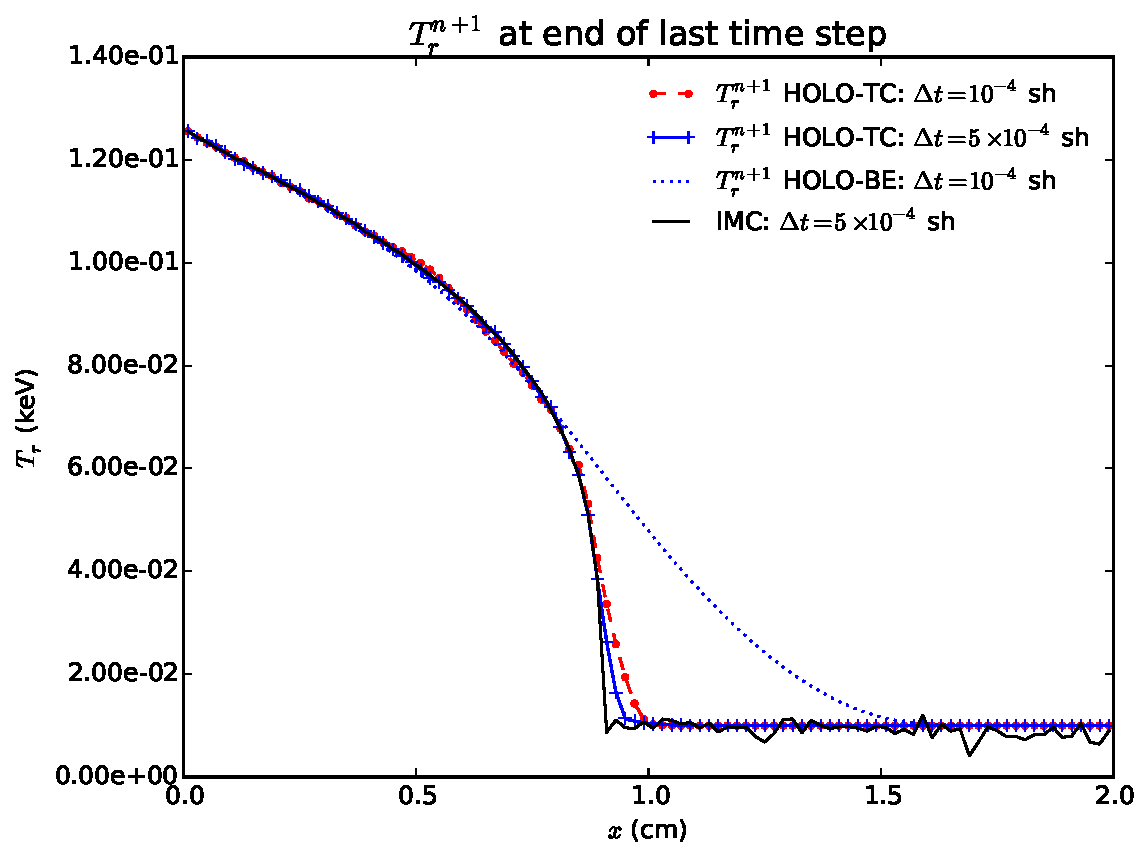
\includegraphics[width=0.92\linewidth]{thin_temp_compare.pdf}
    \caption{\label{fig:thin_temp_compare} Comparison of radiation temperatures for optically thin
        problem. }
\end{figure}

Table.~\ref{tab:fom_thin} compares FOM values for the census
radiation energy densities, for two different $\Delta t$ values.  HOLO results were
generated for the case of 1 and 2 uniform batches, with the same
total number of histories per time step.  At low particle counts for the larger time step
size, the HOLO-TC method
demonstrates substantial noise, leading to instabilities.  This is due to the trial space representation of the
census particles at the end of the time step being poorly estimated.  For the 2 batch
case, the estimate from the first batch leads to less error in the census estimate as the
ECMC solves are simply solving for the deviation from the time-averaged quantities of the first
batch.   At smaller time-steps there
is an increase in statistical efficiency, however the accuracy is reduced due to an
increase in projection error. A finer mesh size is needed to produce higher accuracy.

%The accuracy of the HOLO-ECMC method was compared to a reference solution from IMC. This
%problem is thin enough that we expect IMC to be accuracy with sufficient particle
%histories.  The
%reference solution is the average of 20 IMC simulations of $20\times10^6$
%histories, each with $\delta t =10^{-4}$ sh.  The estimated value of $\ss$ for the
%reference solution is 0.025\%.  The L$_2$ norm of the error in cell-averaged mean
%intensities is computed 
%at the end of the last time step, was computed.  The average over 20 simulations is then
%computed to provide the metric
%\begin{equation}
%    \|e\|^l = \left({\frac{\sum\limits_{i=1}^{N_c}
%    \left(\phi_i^{n+1,l} - \phi_i^{n+1,ref}
%\right)^2}{\sum\limits_{i=1}^{N_c}\left(\phi_i^{n+1,ref}\right)^2}}\right)^{1/2},
%\end{equation}
%where $\phi_i^{n+1,l}$ is the cell-averaged scalar intensity at the end of the last time
%step from the $l$'th independent simulation.  The sample mean of $\|e\|$ from 20
%independent simulations provides a metric for the accuracy of a particular simulation:
%\begin{equation}
%    \overline{\|e\|} = \frac{1}{20}\sum_{l=1}^{20} \|e\|^l
%\end{equation}

\begin{table}
\centering
\caption{\label{tab:fom_thin} {Comparison of FOM for the optically
    thin problem.  Simulation end time is $t=0.003$ sh. The numbers in parenthesis indicate number of
batches per time step.}}
\begin{tabular}{|c|ccc|}\cline{2-4}
    \multicolumn{1}{c|}{}       &
    \multicolumn{3}{|c|}{\FOM} \\ \hline
    \multicolumn{4}{|c|}{$\Delta t = 5\times10^{-4}$ sh} \\\hline
hists./step   &   IMC   & HOLO-TC(1) & HOLO-TC(2) \\ \hline
   30,000     &   1.00  & 0.03  &  0.31      \\
  300,000     &   0.93  & 1.38  &  1.65     \\ 
  1,000,000   &   1.10  & 3.42  &  2.00      \\ \hline
    \multicolumn{4}{|c|}{$\Delta t = 10^{-4}$ sh} \\\hline
hists./step   &  IMC   & HOLO-TC(1) & HOLO-TC(2) \\ \hline
   30,000     &  1.00  &  42.00    & 6.95    \\
  300,000     &  0.98  &  94.47    & 12.38    \\ 
  1,000,000   &  1.11  &  94.85    & 12.00   \\ \hline
\end{tabular}
\end{table}

\subsection{Marshak Wave Problem}

This problem has the same material properties as the optically thin problem except
$\sigma_a(T) = 0.001 T^{-3}$, and the initial temperature is $2.5\times10^{-5}$ keV.  The time step size is linearly increased from $0.001$ sh to a
maximum step of 0.01 sh over the first 10 time steps; the last time step is adjusted to
reach the desired end time of $3.0$ sh.  It was found for this problem that it was
necessary to use more than one batch for the HOLO-TC algorithm to stably converge.
This is because few particles reach $t^{n+1}$ in optically
thick regions.

Although not shown, for $10^6$ histories and 200 mesh cells, there was good agreement
between the HOLO-BE, HOLO-TC, and IMC methods; this problem can be accurately modeled with
the BE time
discretization, but the MC time closure demonstrates stability in a mix of optically thick
and thin regions that occur as the material heats up behind the wave.
Table~\ref{tab:marshak_cont} compares sample statistics for IMC and the HOLO method with
continuous time treatment and for a BE discretization. The HOLO-TC is not as statistically
efficient as HOLO-BE for this problem, but is more efficient than IMC with
sufficient histories.  

\begin{table}[H]
\centering
\caption{\label{tab:marshak_cont} {Comparison of FOM for the Marshak
    wave problem.  Simulation end time is $\mathbf{t=3.0}$ sh.}}
\begin{tabular}{|c|ccc|}\cline{2-4}
    \multicolumn{1}{c|}{}        &
    \multicolumn{3}{|c|}{\FOM} \\ \hline
hists./step    &  IMC   & HOLO-TC (2) & HOLO-BE (2) \\ \hline
  300,000      &  1.00  &   0.43    & 2050          \\  
  1,000,000    &  0.94  &  15.95    & 1806          \\ \hline
\end{tabular}
\end{table}


%%%%%%%%%%%%%%%%%%%%%%%%%%%%%%%%%%%%%%%%%%%%%%%%%%%%%%%%%%%%%%%%%%%%%%%%%%%%%%%%
\section{Conclusions}

Initial results demonstrate that residual MC methods can be extended to include
the time variable, increasing accuracy in optically thin regions compared to a
BE discretization.   Our ECMC algorithm can be more statistically efficient
than IMC, with sufficient batch sizes, although sufficient mesh resolution is needed to limit projection
error between time steps.  We have demonstrated a new approach to
closing the LO equations in time that produces consistent solutions. Long-term, an ideal solution
would require no projection between time step, which will likely require an operator split
on the time derivative.

At this point, we believe that the SDD trial space in time suffers from inaccuracy because particles must
reach the end-of-time step to estimate $I^{n+1}$ and the flat representation over a time step.  Alternatively, the LDFE trial space
could also include the time variable (i.e., it is linear in time).  This has the added
benefit that the slope can be estimated over the interior of the time-step, so all
particle tracks contribute to the estimator.  However, there is some additional truncation
error as the end of time-step is an extrapolated quantity.  This trial space requires substantial modifications to the residual sampling
algorithm because analytic L$_1$ integrals of the local residuals become untenable.  An
importance sampling methodology has been developed but remains to be implemented.  Additionally, modifications to the sampling
algorithm are necessary to extend to higher spatial dimensions or polynomial order, so determining if our
approach is efficient will be beneficial to future work. We plan to include results
for the LDFE time representation for the full paper. 



%%%%%%%%%%%%%%%%%%%%%%%%%%%%%%%%%%%%%%%%%%%%%%%%%%%%%%%%%%%%%%%%%%%%%%%%%%%%%%%%
\bibliographystyle{ans}
\bibliography{references}
\end{document}

